\documentclass[12pt, letterpaper] {article}
\usepackage{graphicx} % Required for inserting images
\usepackage[utf8]{inputenc}
\usepackage[margin=1in]{geometry}
\usepackage{amsmath}
\usepackage{amssymb}
\usepackage{hyperref}
\usepackage{graphicx}
\usepackage{caption}
\usepackage{wasysym}
\setlength{\parindent}{0em}
\setlength{\parskip}{0.5em}

% The following parameters seem to provide a reasonable page setup.
\topmargin 0.0cm
\oddsidemargin 0.2cm
\textwidth 16cm 
\textheight 21cm
\footskip 1.0cm




\title{Tidal Evolution of the Earth-Moon System}
\author{Haobo Yuan}
\date{May 18 2024}

\begin{document}

\maketitle

\section{Introduction}
Throughout history and across cultures, whenever night falls, people have always looked up at the moon, admiring its beautiful moonlight. Poets have also left behind praises and reflections on the moon:
\vspace{12pt}

"The moon, like a flower in heaven's high bower, with silent delight, sits and smiles on the night." -- William Blake
\vspace{12pt}

"Today's people cannot see the ancient moon, but today's moon has shone upon the ancient people." -- Li Bai
\vspace{12pt}

But when did the moon climb into the sky?
\vspace{12pt}

The evolution of the Earth-Moon system is a complex and ancient issue involving knowledge from multiple fields such as celestial mechanics, earth sciences, and astronomy. The goal of this project is to explore the evolution process of the Earth-Moon system. We aim to construct a reliable and efficient model through numerical calculations and computer simulations, simulating the motion of the Earth and the Moon, orbital changes, and possible evolutionary paths. Through this work, we will gain insight into the evolution process of the Earth-Moon system, providing new perspectives and explanations for the origin, formation, and evolution of the moon.
\clearpage


\section{Questions}
\begin{enumerate}

    \item Opt for the CGS unit system. Import Astropy to assign units to each value using \texttt{u.}. Note that some units may not be in the CGS system. To address this, utilize the \texttt{.to} function to convert them to the desired unit. For example, if Earth's radius is $R_{\oplus} = 6371 \, \text{km}$ using Astropy's \texttt{u.km}, then $R_{\oplus} = 6371 \, \text{km}$. Use \textit{${R_{\oplus}.to(u.cm)}$} to convert kilometers to centimeters.
    \vspace{12pt}

    To calculate $L_\oplus$, $S_\oplus$ and $L_{\leftmoon}$ we can plug in the constants we have and set $a_{\leftmoon(0)}$ as $a_{\leftmoon}$  into the following equations
    \begin{eqnarray}
        L_\oplus &=& M_\oplus\sqrt{G(M_\odot + M_\oplus) a_\oplus},\\
        S_\oplus &=& I\Omega_\oplus,\\
        L_{\leftmoon} &=& m_{\leftmoon}\sqrt{G(M_\oplus+m_{\leftmoon})
        a_{\leftmoon}}.
    \end{eqnarray}

    \item To find the present-day values of $T_{\leftmoon}$.  We can use the following equation:
    \begin{equation}
        T_{\leftmoon} = \frac{3}{2}\frac{G m^2_{\leftmoon}}{a_{\leftmoon}}\left(\frac{R_\oplus}{a_{\leftmoon}}\right)^5
        \frac{k_2}{Q_{\leftmoon}}.
    \end{equation}
    
    However, in this equation, $a_{\leftmoon}$ is a variable. We need to define a function called $T_{\text{moon}}$. By substituting the present-day value of the Moon's semi-major axis, we find that $T_{\text{moon}} = 4.5869349 \times 10^{23} \, \text{cm}^2 \, \text{g} \, \text{s}^{-2}$.
    \vspace{12pt}
    
    Notice that since the relation between $T_\oplus$ and $T_{\leftmoon}$ is described as follows  
    $T_{\leftmoon}+T_\odot=T_{\leftmoon}(1+\beta)$, where
    
    \begin{equation}
        \beta = \frac{1}{4.7}  \left(\frac{a_{\leftmoon}}{a_{\leftmoon}(0)}\right)^6.
    \end{equation}
    
    The variable $(a_{\leftmoon})^6$ cancels out; therefore, $T_{\oplus}$ is a constant. 
    
    We find that $T_{\oplus} = 9.759436 \times 10^{22} \, \text{cm}^2 \, \text{g} \, \text{s}^{-2}$.
    
    \clearpage

    \item Start from the following equations:
    \begin{eqnarray}
        \frac{dL_\oplus}{dt} &=& T_\odot,\\
        \frac{dS_\oplus}{dt} &=& -T_\odot-T_{\text{\leftmoon}},\\
        \frac{dL_{\leftmoon}}{dt} &=& T_{\leftmoon}.
    \end{eqnarray}
    
    we can replace \(dt\) with \(\delta t\) and rearrange the equations to obtain that:

    \begin{eqnarray}
        \begin{cases}
            t_{\text{1}} = 2.7144313\times 10^{24} \, \text{s},\\
            t_{\text{2}} = -1.0479156 \times 10^{17} \, \text{s},\\
            t_{\text{3}} = 6.3054784\times 10^{17} \, \text{s}
        \end{cases}
    \end{eqnarray}

    
    \item We can define a function called \texttt{rhs} that provides us with the right-hand side of equations (6), (7), and (8) given time and a parameter vector $\mathbf{W}$, which contains Earth's angular momentum, Earth spin angular momentum, and Moon's angular momentum. To achieve this, we also need an auxiliary function called \texttt{ax} which calculates the semi-major axis distance of the Moon with different Moon's angular momentum.
    
    \item To solve the previous right-hand side function, we need to use \texttt{solve\_ivp} by utilizing the three values we found earlier in 1. as the initial value of the list \textbf{W}, set the time span in seconds and the time step N as a year, which is 31536000 seconds.

    From the results, we obtained that the Moon probably formed around:

    \begin{equation}
        t = \textbf{1.54 billion years ago}.
    \end{equation}
    
    \clearpage
    
    \item A graph showing how the semi-major axis of the Moon changes with time.

    \begin{figure}[h!]
        \centering
        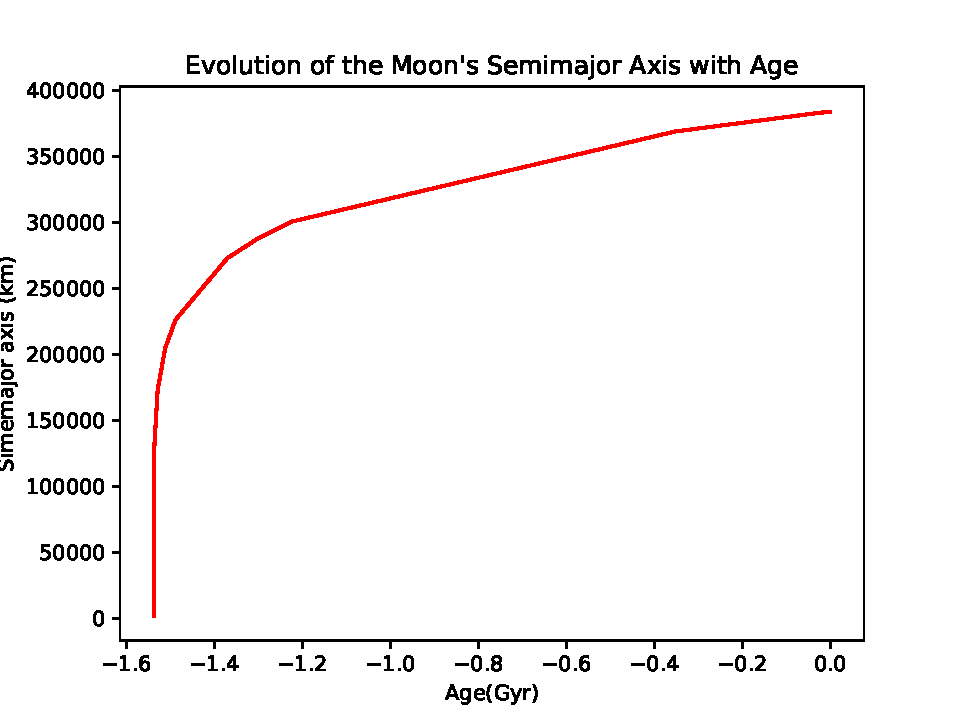
\includegraphics[width=0.45\linewidth, keepaspectratio]{age.pdf}
        \caption{The figure shows when the Moon formed, indicated by when the semi-major axis approaches zero.}
        \label{fig: "Evolution of the Moon's Semimajor Axis with Age"}
    \end{figure}
    
    \item Let's explore the relationship between the length of the day (lod) and Earth's spin angular momentum. We have the following:
    The Earth's moment of inertia is $I = 0.3299M_\oplus R_\oplus^2$. The angular velocity of the Earth is $\Omega_\oplus = \frac{2\pi}{\text{lod}}$, where lod is the length of the sidereal day. From equation (3), we have $S_\oplus = I\Omega_\oplus$, rearrange these equations we will find lod for different Earth spin angular momentum is 
    
    \begin{equation}
        lod = {\frac{{2\pi}{I}}{S_\oplus}}
    \end{equation}
    
    Results of lod as figure 2 shown.

    \begin{figure}[h!]
        \centering
        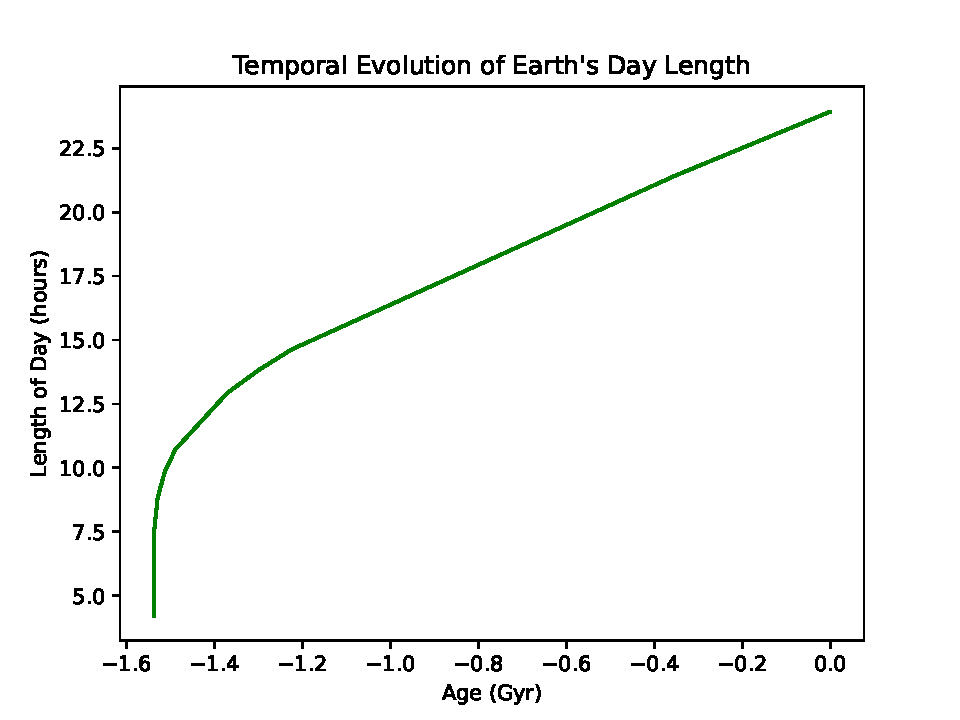
\includegraphics[width=0.45\linewidth, keepaspectratio]{lod.pdf}
        \caption{The figure illustrates how the length of the day changes with different Earth spin angular momentum}
        \label{fig: "Temporal Evolution of Earth's Day Length"}
    \end{figure}

    \clearpage

    \item The Roche Radius, also known as the Roche limit, defines the distance within which a celestial body, held together solely by its own gravity, will disintegrate because the tidal forces from a second celestial body surpass the gravitational self-attraction of the first body. This limit is mathematically expressed by the following expansion:
    
    \begin{equation}
        {\displaystyle d=R_{M}\left(2{\frac {\rho _{M}}{\rho _{m}}}\right)^{\frac {1}{3}}}
    \end{equation}
  
    To find what the Roche radius of the Moon, firstly, we need to find the densities of Earth and the Moon. By substituting those numbers, the Roche radius of the Moon is calculated as follows:
    
    \begin{equation}
        d_{\leftmoon} = 9494.5549\, \text{km}
    \end{equation}
    
    To determine the length of the day at the time when the Moon formed at the Roche radius, we set $a_{\leftmoon} = d_{\leftmoon}$, and by using equation (3), $L_{\leftmoon} = m_{\leftmoon}\sqrt{G(M_{\oplus}+m_{\leftmoon})a_{\leftmoon}}$, we can find the angular momentum of the Moon at the time when it formed. This is given by the following expression:

    \begin{equation}
        L_{\text{moon}}(d) = m_{\text{moon}}\sqrt{G(M_{\oplus}+m_{\text{moon}})d_{\text{moon}}}.
    \end{equation}

    Since angular momentum is conserved, the sum of Earth's spin angular momentum and the Moon's angular momentum is therefore constant. This can be expressed as:
    
    \begin{equation}
        L_{\text{EM}} = s_{\oplus} + L_{\text{moon}}
    \end{equation}

    We can use the initial values of $S_{\oplus}$ and $L_{\text{moon}}$ to determine $L_{\text{EM}}$. Subtracting $L_{\text{moon}}(d)$ from this value gives us $S_{\oplus}(d)$, the spin angular momentum of the Earth when the Moon formed at the Roche radius.

    By utilizing our defined function, we can observe that at that time, the length of the day is:
    
    \begin{equation}
        {lod(d) = 16629.626\, \text{s} = 4.6193407\, \text{hr}}
    \end{equation}
    
    \item We want to verify if the results from this model are consistent with the ages determined for Earth and the Moon. We know that the ages of Earth and the Moon are:

    \begin{equation}
        \begin{cases}
            Age_{\leftmoon} &= 4.35\, \text{billion years}, \\
            Age_{\oplus} &= 4.54\, \text{billion years}
        \end{cases}
    \end{equation}

    Unfortunately, our model did not produce results close to those obtained by radiometric dating of rocks.
 
\end{enumerate}

\section{Thinking}
Given the significant discrepancy of approximately 3 Gyr in the results obtained by our model, it is imperative to address potential sources of error.

Firstly, it is necessary to carefully examine the accuracy of the tidal equations used in our model. The precision of our constants is uncertain, raising questions about their reliability. Given that we are dealing with an initial value problem, it is pertinent to emphasize the sensitivity to initial conditions. Any differences in initial parameters could lead to significant deviations in the final results. Additionally, the influence of external factors such as the passage of comets over the 3 Gyr time scale may alter the tidal equations, thereby affecting the accuracy of our model. Further validation is warranted.

Secondly, the validity of estimates regarding the ages of the Earth and the Moon merits further investigation. Inaccuracies in these estimates could contribute to the observed disparities in results. One potential factor influencing these estimates is the potential contamination of test rocks used for dating. Moreover, inherent limitations associated with sampling may not adequately represent the entire Earth and could distort the results.

\section{References}

\begin{itemize}

    \item 
    U.S. Geological Survey 1997, Age of the Earth, \url{https://pubs.usgs.gov/gip/geotime/age.html}

    \item 
    Dalrymple, G. Brent 2001, "The age of the Earth in the twentieth century: a problem (mostly) solved," Special Publications, Geological Society of London, 190, 205-221, \url{https://doi.org/10.1144/GSL.SP.2001.190.01.14}

    \item 
    National Aeronautics and Space Administration (NASA), Moon Fact Sheet, \url{https://nssdc.gsfc.nasa.gov/planetary/factsheet/moonfact.html}

    \item 
    National Aeronautics and Space Administration (NASA), Earth Fact Sheet, \url{https://nssdc.gsfc.nasa.gov/planetary/factsheet/earthfact.html}

    \item 
    Borg, L. E., Gaffney, A. M., and Shearer, C. K. 2015, "A review of lunar chronology revealing a preponderance of 4.34–4.37 Ga ages," Meteoritics and Planetary Science, 50, 715-732, \url{https://doi.org/10.1111/maps.12371}
    
\end{itemize}

\end{document}




